\section{EXIST}
%Descripción de la tarea
\begin{frame}{Task description}
  
\begin{columns}
\column{0.6\textwidth}
\begin{itemize}
    \item 4th edition of EXIST
    \item Sexism identification and categorization in text/memes
    \item LeWiDi framework + \textbf{memes tasks}
    \item 6 tasks (\textit{Tweets} + \textbf{Memes}) grouped in the same taxonomy:
    \begin{itemize}
        \item Sexism Identification (1 and \textbf{4})
        \item Source Intention (2 and \textbf{5})\footnote{Task 2 for tweets contains an extra category}
        \item Sexism Categorization (3 and \textbf{6})
    \end{itemize}
\end{itemize}
\column{0.4\textwidth}
\centering
\includesvg[width=0.9\textwidth]{images/EXIST-TAREAS.svg}
\begin{table}[]
    \huge
    \resizebox{\textwidth}{!}{
    \begin{tabular}{|c|c|c|}
    \hline
    Task                  & Hard evaluation   & Soft evaluation             \\ \hline
    Sexism Identification & \textbf{ICM, ICM Norm}, F1 & \textbf{ICM Soft, ICM Soft Norm}, CE \\ \hline
    Source Intention      & \textbf{ICM, ICM Norm}, F1 & \textbf{ICM Soft, ICM Soft Norm}, CE \\ \hline
    Sexism Categorization & \textbf{ICM, ICM Norm}    & \textbf{ICM Soft, ICM Soft Norm}     \\ \hline
    \end{tabular}
    }
\end{table}
\end{columns}
\footfullcite{Plaza2024OverviewOE}  
\end{frame}

\begin{frame}{Sexism identification: examples}
    \begin{columns}
        \column{0.5\textwidth}
        \centering
        No stereotype
        
\includegraphics[width=\textwidth]{images/110056.jpeg}
        \column{0.5\textwidth}
        \centering
        Stereotype
        
\includegraphics[width=\textwidth]{images/110061.jpeg}
    \end{columns}
\end{frame}

\begin{frame}{Source intention: examples}
\begin{columns}
    \column{0.5\textwidth}
    \centering
    Direct
    
\includegraphics[width=\textwidth]{images/110070.jpeg}
    \column{0.5\textwidth}
    \centering
    Judgmental
    
\includegraphics[width=\textwidth]{images/110015.jpeg}
\end{columns}
\end{frame}

\begin{frame}{Sexism categorization: examples}
\begin{columns}
    \begin{column}{0.33\textwidth}
        \centering
        Ideological and inequality
        
\includegraphics[width=0.9\textwidth]{images/idelogocial.jpeg}
        \vfill
        Stereotyping and dominance
        
\includegraphics[width=0.9\textwidth]{images/dominance.jpeg}
    \end{column}
    \begin{column}{0.33\textwidth}
        \centering
        Objectification
        
\includegraphics[width=0.9\textwidth]{images/Objectification.jpeg}
        \vfill
        Sexual violence
        
\includegraphics[width=0.9\textwidth]{images/sexual-violence.jpeg}
    \end{column}
    \begin{column}{0.33\textwidth}
        \centering
        Misogyny and non-sexual violence
        
\includegraphics[width=0.9\textwidth]{images/violence.jpeg}
    \end{column}
\end{columns}
\end{frame}

\begin{frame}{Dataset}
\only<1>{
    \begin{itemize}
        \item Created by keyword search
        \item Various sources: Google, Twitter, Reddit and Forocoches
        \item English and Spanish
        \item Crowd annotation via Prolific
        \begin{itemize}
            \item 450 annotators for each language
            \item Each sample is annotated by 6 people
            \item 26 annotations on average
            \item Demographic information of each annotator
        \end{itemize}
    \end{itemize}
    \footfullcite{Plaza2024OverviewOE}
}
\end{frame}

\begin{frame}{Dataset (ES)}
    \begin{columns}[T]
        \begin{column}{0.3\textwidth}
            %\centering %Uncomment this line for horizontal centering 
            \centering
            \textbf{Task 4}

            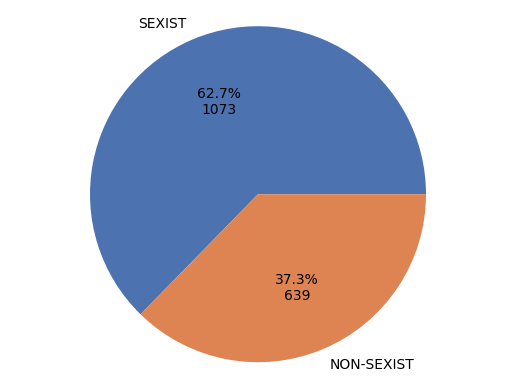
\includegraphics[height=0.4\textheight, width=\textwidth, keepaspectratio]{images/t4_es_hard_presentacion.png}%
            \vfill
            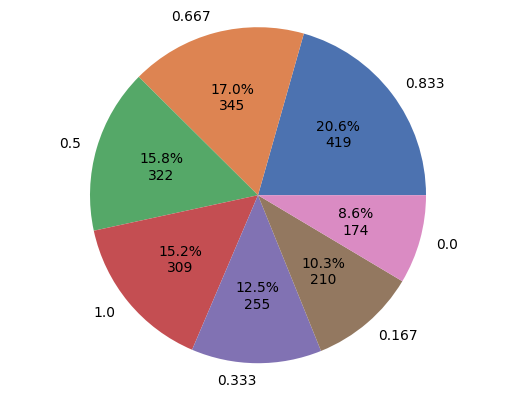
\includegraphics[height=0.4\textheight, width=\textwidth, keepaspectratio]{images/t4_es_soft_presentacion.png}%
        \end{column}

        \begin{column}{0.3\textwidth}
            \centering %Uncomment this line for horizontal centering 
            \textbf{Task 5}

            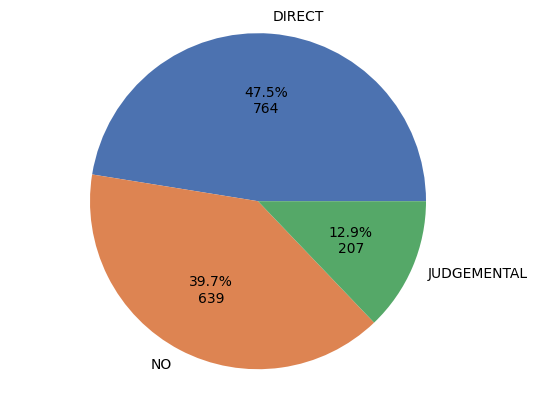
\includegraphics[height=0.4\textheight, width=\textwidth, keepaspectratio]{images/t5_es_hard_presentacion.png}%
            \vfill
            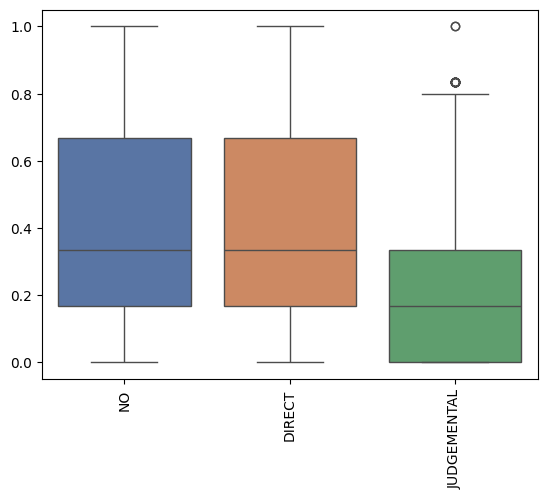
\includegraphics[height=0.4\textheight, width=\textwidth, keepaspectratio]{images/t5_es_soft_presentacion.png}%
        \end{column}

        \begin{column}{0.3\textwidth}
            \centering %Uncomment this line for horizontal centering
            \textbf{Task 6}

            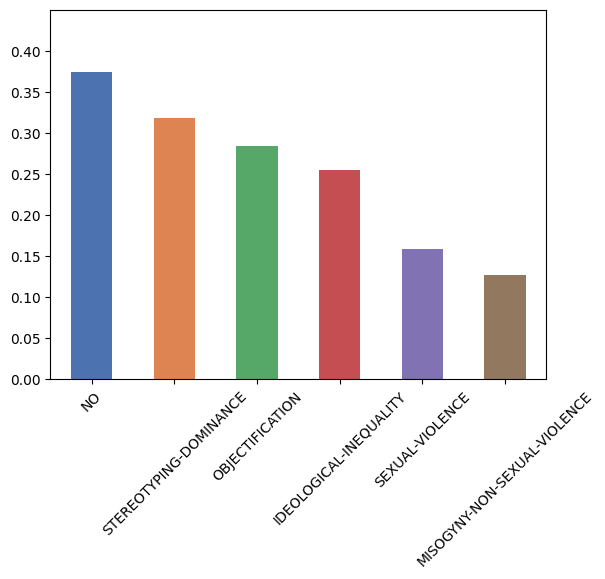
\includegraphics[height=0.4\textheight, width=\textwidth, keepaspectratio]{images/t6_es_hard_presentacion.png}%
            \vfill
            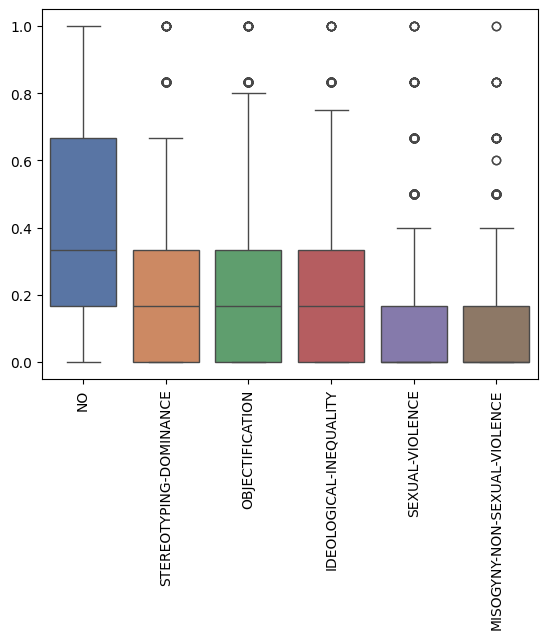
\includegraphics[height=0.4\textheight, width=\textwidth, keepaspectratio]{images/t6_es_soft_presentacion.png}%
        \end{column}
    \end{columns}
\end{frame}

\begin{frame}{Dataset (EN)}
    \begin{columns}[T]
        \begin{column}{0.3\textwidth}
            %\centering %Uncomment this line for horizontal centering 
            \centering
            \textbf{Task 4}

            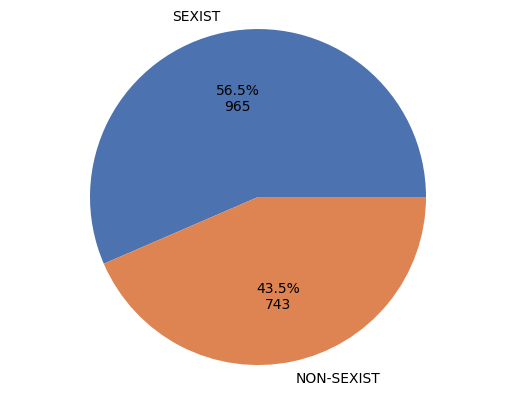
\includegraphics[height=0.4\textheight, width=\textwidth, keepaspectratio]{images/t4_en_hard_presentacion.png}%
            \vfill
            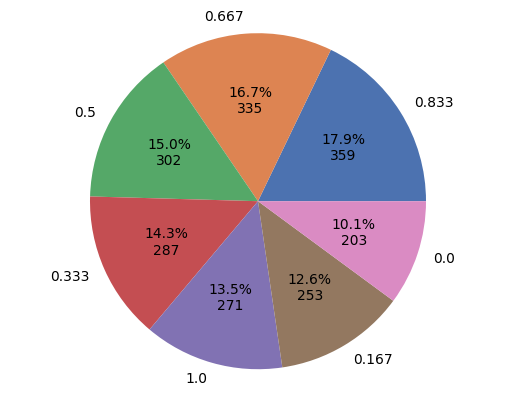
\includegraphics[height=0.4\textheight, width=\textwidth, keepaspectratio]{images/t4_en_soft_presentacion.png}%
        \end{column}

        \begin{column}{0.3\textwidth}
            \centering %Uncomment this line for horizontal centering 
            \textbf{Task 5}

            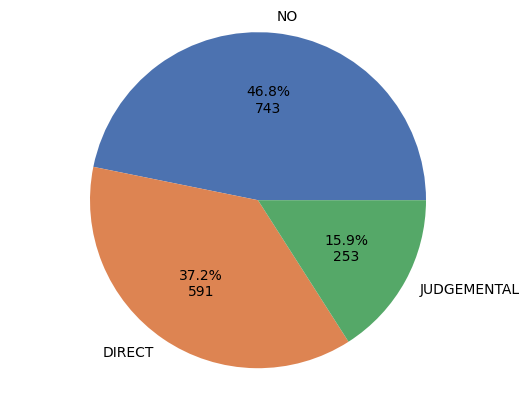
\includegraphics[height=0.4\textheight, width=\textwidth, keepaspectratio]{images/t5_en_hard_presentacion.png}%
            \vfill
            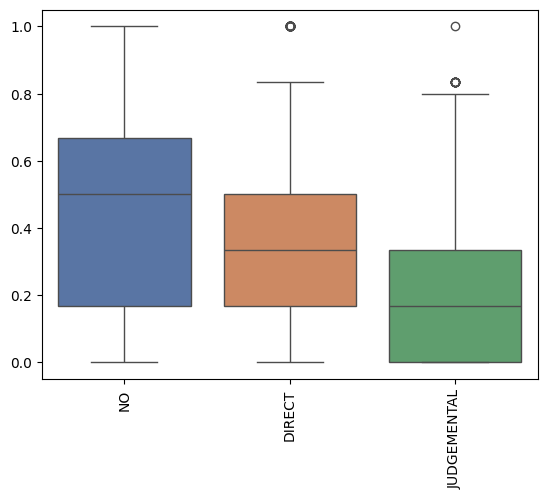
\includegraphics[height=0.4\textheight, width=\textwidth, keepaspectratio]{images/t5_en_soft_presentacion.png}%
        \end{column}

        \begin{column}{0.3\textwidth}
            \centering %Uncomment this line for horizontal centering
            \textbf{Task 6}

            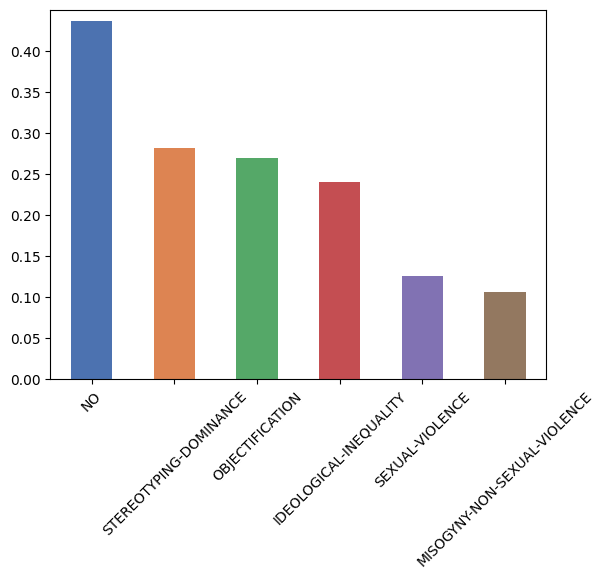
\includegraphics[height=0.4\textheight, width=\textwidth, keepaspectratio]{images/t6_en_hard_presentacion.png}%
            \vfill
            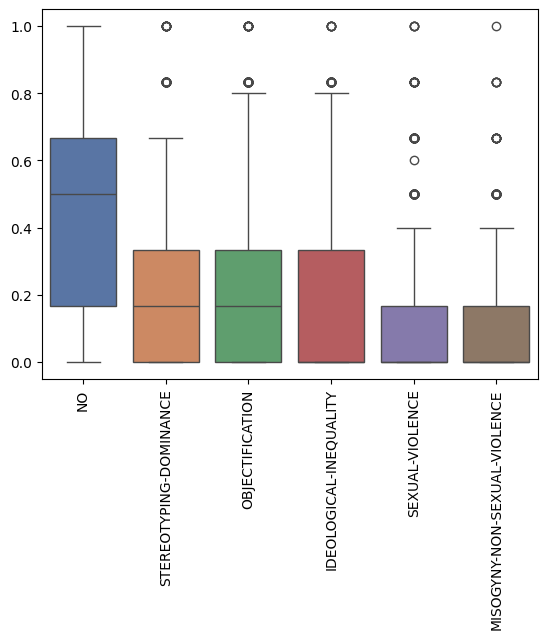
\includegraphics[height=0.4\textheight, width=\textwidth, keepaspectratio]{images/t6_en_soft_presentacion.png}%
        \end{column}
    \end{columns}
\end{frame}
%Propuesta del sistema
\begin{frame}{System proposals}

\begin{columns}
    \column{0.5\textwidth}
        \begin{itemize}
            \item Comparison of different modalities:
                \begin{itemize}
                    \item Unimodal architectures: \textit{Transformer encoder} (RoBERTa and ViT)
                    \item Multimodal architecture: \textit{Early fusion} by concatenating the [CLS] token
                \end{itemize}
            \item LeWiDi approaches:
                \begin{itemize}
                    \item Hard label
                    \item Soft label
                    \item \textbf{\textit{Why no multi-task approach?}}
                \end{itemize}
            \item One model for each language 
    \end{itemize}
    \column{0.5\textwidth}
    \centering
    \includesvg[width=0.8\textwidth]{images/unimodal.svg}
    \includesvg[width=0.45\textwidth]{images/early_fusion.svg}
\end{columns}
\end{frame}


\begin{frame}{Enhancing textual modality performance}
    \begin{columns}
        \column{0.5\textwidth}
        \centering 
        \begin{itemize}
            \item Textual preprocessing to remove noise (watermarks, emojis, URLS...)
            \item Avoid biases by masking \textit{identity term} 
            \item \textbf{Closing the visual and textual gap: meme descriptions (LLaVa)}
            \item \textbf{Data augmentation by incorporating tweets on the training dataset} \footnote{Available on text-only. Task 5 avoided.}
        \end{itemize}
        \column{0.5\textwidth}
        \centering
        \begin{figure}
            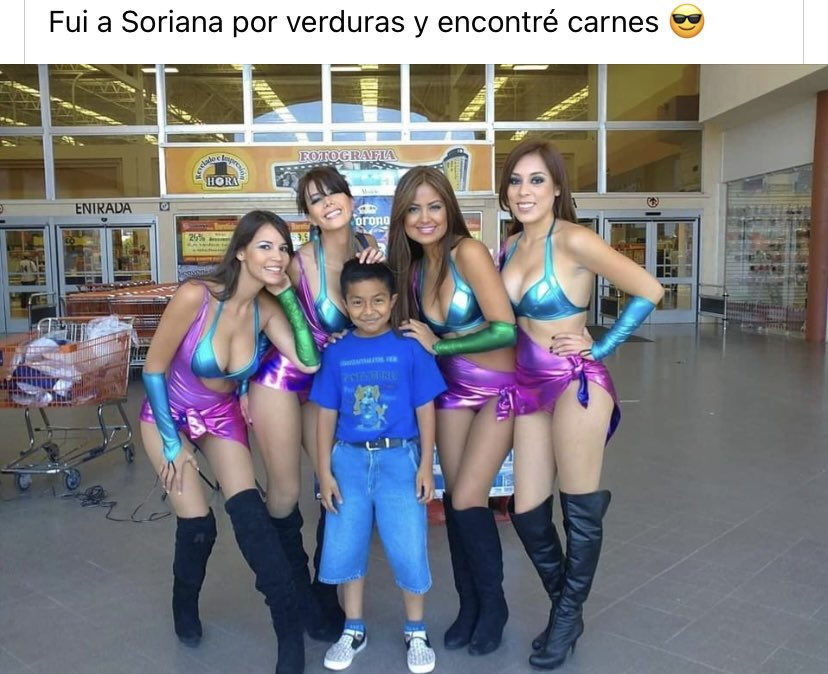
\includegraphics[width=\textwidth]{images/111702.jpeg}
            \caption{A group of women and a children pose for a photo.}
        \end{figure}
    \end{columns}

\end{frame}


%Resultados T4
\begin{frame}{Task 4: Sexism Identification in Memes}
\only<1>{
\begin{table}[]
\centering
\begin{adjustbox}{width=0.95\textwidth}
\begin{tabular}{|c|c|c|c|c|c|}
\hline
Architecture                                                                     & Label & Ranking     & ICM $\uparrow$ & ICM Norm $\uparrow$ & F1 - Sexist $\uparrow$ \\ \hline
\multirow{2}{*}{Text + CTXT}                                                    & Hard  & 14          & 0.087          & 0.544               & 0.729                  \\ \cline{2-6} 
                                                                                 & Soft  & 13          & 0.088          & 0.545               & 0.697                  \\ \hline
\multirow{2}{*}{\begin{tabular}[c]{@{}c@{}}Text + CTXT +\\ Tweets\end{tabular}} & Hard  & 29          & -0.093         & 0.453               & 0.684                  \\ \cline{2-6} 
                                                                                 & Soft  & 8           & 0.104          & 0.553               & 0.716                  \\ \hline
\multirow{2}{*}{Image}                                                           & Hard  & 43          & -0.312         & 0.341               & 0.677                  \\ \cline{2-6} 
                                                                                 & Soft  & 45          & -0.359         & 0.317               & 0.640                  \\ \hline
\multirow{2}{*}{Early}                                                           & Hard  & $4^\dagger$ & \textbf{0.166} & \textbf{0.584}      & \textbf{0.736}         \\ \cline{2-6} 
                                                                                 & Soft  & 34          & -0.165         & 0.416               & 0.652                  \\ \hline \hline
Gold Baseline                                                                    & -     & 0           & 0.983          & 1.000               & 1.000                  \\ \hline
Ganadores                                                                        & -     & 1           & 0.318          & 0.662               & 0.764                  \\ \hline
\end{tabular}%
\end{adjustbox}
\caption{Test results for the hard evaluation in task 4 of EXIST. In bold, our best results by metric. $\dagger$ denotes our best ranking.}
\label{tab:exist_t4_hard}
\end{table}
\footfullcite{Plaza2024OverviewOE}
}

\only<2>{
\begin{table}[]
\centering
\begin{adjustbox}{width=0.95\textwidth}

\begin{tabular}{|c|c|c|c|c|c|}
\hline
Architecture                                                                     & Label & Ranking     & ICM Soft $\uparrow$ & ICM Soft Norm $\uparrow$ & \textit{Cross Entropy} $\downarrow$ \\ \hline
\multirow{2}{*}{Text + CTXT}                                                    & Hard  & 2           & -0.201              & 0.468                    & 0.969                               \\ \cline{2-6} 
                                                                                 & Soft  & 25          & -0.679              & 0.391                    & 0.925                               \\ \hline
\multirow{2}{*}{\begin{tabular}[c]{@{}c@{}}Text + CTXT +\\ Tweets\end{tabular}} & Hard  & 17          & -0.546              & 0.412                    & 1.077                               \\ \cline{2-6} 
                                                                                 & Soft  & 11          & -0.430              & 0.431                    & \textbf{0.918}                      \\ \hline
\multirow{2}{*}{Image}                                                           & Hard  & 27          & -0.947              & 0.348                    & 1.033                               \\ \cline{2-6} 
                                                                                 & Soft  & 34          & -1.160              & 0.314                    & 1.015                               \\ \hline
\multirow{2}{*}{Early}                                                           & Hard  & $1^\dagger$ & \textbf{-0.118}     & \textbf{0.481}           & 1.081                               \\ \cline{2-6} 
                                                                                 & Soft  & 26          & -0.869              & 0.360                    & 0.980                               \\ \hline \hline
Gold Baseline                                                                    & -     & 0           & 3.111               & 1.000                    & 0.585                               \\ \hline
Ganadores                                                                        & -     & 1           & -0.293              & 0.453                    & 1.103                               \\ \hline
\end{tabular}%

\end{adjustbox}
\caption{Test results for the soft evaluation in task 5 of EXIST. In bold, our best results by metric. $\dagger$ denotes our best ranking.}
\label{tab:exist_task4_soft}
\end{table}
\footfullcite{Plaza2024OverviewOE}
}
\end{frame}

%Resultados T5
\begin{frame}{Task 5: Source Intention in Memes}

\only<1>{
\begin{table}[]
\centering
\begin{adjustbox}{width=0.95\textwidth}
    \begin{tabular}{|c|c|c|c|c|c|}
        \hline
        Architecture                  & Label & Ranking     & ICM $\uparrow$  & ICM Norm $\uparrow$ & F1 - Sexist $\uparrow$ \\ \hline
        \multirow{2}{*}{Text + CTXT} & Hard  & 6           & -0.272          & 0.406               & 0.382                  \\ \cline{2-6} 
                                      & Soft  & $1^\dagger$ & \textbf{-0.207} & \textbf{0.428}      & 0.400                  \\ \hline
        \multirow{2}{*}{Image}        & Hard  & 16          & -0.654          & 0.273               & 0.294                  \\ \cline{2-6} 
                                      & Soft  & 20          & -0.752          & 0.239               & 0.315                  \\ \hline
        \multirow{2}{*}{Early}        & Hard  & 13          & -0.360          & 0.375               & 0.377                  \\ \cline{2-6} 
                                      & Soft  & 2           & -0.237          & 0.418               & \textbf{0.411}         \\ \hline \hline
        Gold Baseline                 & -     & 0           & 1.438           & 1.000               & 1.000                  \\ \hline
        Ganadores                     & -     & 1           & -0.240          & 0.417               & 0.387                  \\ \hline
        \end{tabular}%
\end{adjustbox}
\caption{Test results for the hard evaluation in task 5 of EXIST. In bold, our best results by metric. $\dagger$ denotes our best ranking.}
\label{tab:exist_t5_hard}
\end{table}
\footfullcite{Plaza2024OverviewOE}
}

\only<2>{
\begin{table}[]
\centering
\begin{adjustbox}{width=\textwidth}
    \begin{tabular}{|c|c|c|c|c|c|}
        \hline
        Architecture                  & Label & Ranking     & ICM Soft $\uparrow$ & ICM Soft Norm $\uparrow$ & \textit{Cross Entropy} $\downarrow$ \\ \hline
        \multirow{2}{*}{Text + CTXT} & Hard  & $3^\dagger$ & \textbf{-1.323}     & \textbf{0.359}           & 1.602                               \\ \cline{2-6} 
                                      & Soft  & 8           & -1.620              & 0.328                    & 1.449                               \\ \hline
        \multirow{2}{*}{Image}        & Hard  & 10          & -1.969              & 0.291                    & 1.565                               \\ \cline{2-6} 
                                      & Soft  & 13          & -2.012              & 0.286                    & 1.512                               \\ \hline
        \multirow{2}{*}{Early}        & Hard  & 9           & -1.620              & 0.328                    & 1.520                               \\ \cline{2-6} 
                                      & Soft  & 5           & -1.377              & 0.354                    & \textbf{1.434}                      \\ \hline \hline
        Gold Baseline                 & -     & 0           & 4.702               & 1.000                    & 0.933                               \\ \hline
        Ganadores                     & -     & 1           & -1.245              & 0.368                    & 1.624                               \\ \hline
        \end{tabular}%
\end{adjustbox}
\caption{Test results for the soft evaluation in task 5 of EXIST. In bold, our best results by metric. $\dagger$ denotes our best ranking.}
\label{tab:exist_t5_soft}
\end{table}
\footfullcite{Plaza2024OverviewOE}
}

\end{frame}

%Resultados T6
\begin{frame}{Task 6: Sexism Categorization in Memes}
    \only<1>{
    \begin{table}[]
    \begin{adjustbox}{width=0.95\textwidth}
        \begin{tabular}{|c|c|c|c|c|c|}
            \hline
            Architecture                                                                     & Label & Ranking     & ICM $\uparrow$  & ICM Norm $\uparrow$ & F1 - Sexist $\uparrow$ \\ \hline
            \multirow{2}{*}{Text + CTXT}                                                    & Hard  & $2^\dagger$ & \textbf{-0.783} & \textbf{0.338}      & 0.402                  \\ \cline{2-6} 
                                                                                             & Soft  & 5           & -0.853          & 0.323               & 0.380                  \\ \hline
            \multirow{2}{*}{\begin{tabular}[c]{@{}c@{}}Text + CTXT +\\ Tweets\end{tabular}} & Hard  & 8           & -1.057          & 0.281               & 0.387                  \\ \cline{2-6} 
                                                                                             & Soft  & 3           & -0.810          & 0.332               & \textbf{0.434}         \\ \hline
            \multirow{2}{*}{Image}                                                           & Hard  & 20          & -1.647          & 0.158               & 0.222                  \\ \cline{2-6} 
                                                                                             & Soft  & 21          & -1.652          & 0.157               & 0.202                  \\ \hline
            \multirow{2}{*}{Early}                                                           & Hard  & 11          & -1.212          & 0.249               & 0.289                  \\ \cline{2-6} 
                                                                                             & Soft  & 12          & -1.270          & 0.237               & 0.316                  \\ \hline \hline
            Gold Baseline                                                                    & -     & 0           & 2.410           & 1.000               & 1.000                  \\ \hline
            Ganadores                                                                        & -     & 1           & -0.700          & 0.355               & 0.432                  \\ \hline
            \end{tabular}%
    \end{adjustbox}
    \caption{Test results of the hard evaluation in task 6 of EXIST. In bold, our best results by metric. $\dagger$ denotes our best ranking.}
    \label{tab:exist_t6_hard}
    \end{table}
    \footfullcite{Plaza2024OverviewOE}
    }
    \only<2>{
    \begin{table}[]
    \centering
    \begin{adjustbox}{width=0.95\textwidth}
        \begin{tabular}{|c|c|c|c|c|}
            \hline
            Architecture                                                                     & Label & Ranking     & ICM Soft $\uparrow$ & ICM Soft Norm $\uparrow$ \\ \hline
            \multirow{2}{*}{Text + CTXT}                                                    & Hard  & 9           & -5.737              & 0.196                    \\ \cline{2-5} 
                                                                                             & Soft  & 2           & -4.609              & 0.256                    \\ \hline
            \multirow{2}{*}{\begin{tabular}[c]{@{}c@{}}Text + CTXT +\\ Tweets\end{tabular}} & Hard  & 20          & -8.080              & 0.072                    \\ \cline{2-5} 
                                                                                             & Soft  & $1^\dagger$ & \textbf{-4.310}     & \textbf{0.272}           \\ \hline
            \multirow{2}{*}{Image}                                                           & Hard  & 11          & -6.411              & 0.160                    \\ \cline{2-5} 
                                                                                             & Soft  & 14          & -6.519              & 0.155                    \\ \hline
            \multirow{2}{*}{Early}                                                           & Hard  & 7           & -5.472              & 0.210                    \\ \cline{2-5} 
                                                                                             & Soft  & 8           & -5.550              & 0.206                    \\ \hline \hline
            Gold Baseline                                                                    & -     & 0           & 9.434               & 1.000                    \\ \hline
            Ganadores                                                                        & -     & 1           & -4.904              & 0.245                    \\ \hline
            \end{tabular}%
    \end{adjustbox}

    
    \caption{Test results of the soft evaluation in task 6 of EXIST. In bold, our best results by metric. $\dagger$ denotes our best ranking.}
    \label{tab:t6_exist_soft}
    \end{table}
    \footfullcite{Plaza2024OverviewOE}
    }
\end{frame}